\documentclass[12pt]{article}
\usepackage[spanish]{babel}
\usepackage{geometry}
\geometry{a4paper, margin=1in}
\usepackage{graphicx}
\usepackage{xcolor}
\usepackage{titlesec}
\usepackage{parskip}
\usepackage{multicol}
\usepackage{cite}

\definecolor{highlight}{RGB}{255, 255, 0}

\titleformat{\section}{\normalfont\Large\bfseries}{\thesection}{1em}{}
\titleformat{\subsection}{\normalfont\large\bfseries}{\thesubsection}{1em}{}

\begin{document}

% Logos
\begin{minipage}{0.45\textwidth}
    
\includegraphics[width=0.4\textwidth]{inFiles/Figures/epnLogo.jpg}
\end{minipage}
\hfill
\begin{minipage}{0.45\textwidth}
    \raggedleft
    
\includegraphics[width=0.4\textwidth]{inFiles/Figures/FIS_logo.jpg}
\end{minipage}

\vspace{0.5cm}

% Títulos principales
\begin{center}
    \textbf{ESCUELA POLITÉCNICA NACIONAL}\\[0.2cm]
    \textbf{FACULTAD DE INGENIERÍA DE SISTEMAS}\\[0.2cm]
    \textbf{INGENIERÍA {\textbf{EN COMPUTACION}}}
\end{center}

\vspace{0.5cm}
\hrule
\vspace{0.5cm}

% Datos principales
\noindent\textbf{PERÍODO ACADÉMICO:} 2025-A\\[0.2cm]
\noindent\textbf{ASIGNATURA:} ICCD412 Métodos Numéricos \hfill \textbf{GRUPO:} GR2\\[0.2cm]
\noindent\textbf{TIPO DE INSTRUMENTO:} {Deber N°6}\\[0.2cm]
\noindent\textbf{FECHA DE ENTREGA LÍMITE:} {09/05/2025}\\[0.2cm]
\noindent\textbf{ALUMNO:} {Lema Luis}

\vspace{0.5cm}
\hrule
\vspace{1cm}


% Secciones
\section*{TEMA}
{Método de la secante}

\vspace{0.5cm}

\section*{OBJETIVOS}
\begin{itemize}
    \item { Aplicar el método de la secante para encontrar una raíz de la ecuación 
    cos x =x , iniciando con dos valores cercanos y deteniéndose cuando la diferencia entre 
    aproximaciones sea menor que $10^{-16}$}

\end{itemize}

\vspace{0.5cm}

\section*{DESARROLLO}


\begin{minipage}{0.95\textwidth}
    \raggedleft
    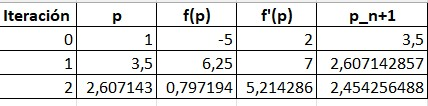
\includegraphics[width=1.15\textwidth]{inFiles/Figures/eje1.jpg}
\end{minipage}

\vspace{0.5cm}


\section*{CONCLUSIONES}
\begin{itemize}
    \item {El método de la secante funcionó bastante bien y en solo 8 pasos 
    ya teníamos una solución muy precisa. A partir de ahí, la diferencia entre valores fue tan pequeña 
    que la hoja de cálculo ya no pudo seguir, lo cual indica que se alcanzó la raíz con la precisión solicitada}

    \item {Me pareció interesante ver cómo el método se detuvo naturalmente cuando ya no podía mejorar más la respuesta. 
    Esto demuestra que el criterio de parada con $10^{-16}$ funciona como un buen control de precisión y evita hacer cálculos innecesarios}
\end{itemize}


\vspace{0.5cm}


\end{document}
